\subsubsection{Purpose}
A user who successfully creates events may wish to take advantage of one of the most interesting feature of Travlendar+, which concerns both time and itinerary. This makes Travlendar+ an enhanced calendar-based application. Particularly, a user can add as many events as he/she may want, and the system will be responsible to arrange time slots so as to ensure that he/she is never going to be late. The system allows the user to insert the location of the event as well so as to instruct him to take the best itinerary to reach such location. To compute the best route in terms of both space and time a sequence of calculations will be executed. Various factors - both that can be handled by the user and that which cannot - are considered.

\subsubsection{Scenario 1}
Alice is a manager who needs to go often around the city for work to meet customers. Since living in a big city and having to wake up soon, she knows that in the peak hours it's difficult to move around the city, and the system is aware of this too. She often needs to move around the entire city pretty fast. So, whenever she wants to see the task ahead, she knows she is in good hands, in fact the system typically proposes her the best route which consists of taking the bus or the underground train, or - often - a combination of them so that she can avoid the traffic of the city. 
\subsubsection{Scenario 2}
Charlie, who is a little bit messy and unmindful, inserts multiple appointments for work for the current day and fills up the entire time window for which lunch is supposed to be done. Fortunately, the application reminds here not to forget to have lunch so he is prompted with a dialog to choose when he would like to insert lunchtime. Then he adds two appointments which are too close together. Itinerary is calculated anyway, but no feasible route is possible to reach the destination. The system however recognizes that 5 minutes before the end of the first appointment a bus will pass by there, so he is informed that if he desires to be in time to the upcoming event he will just have to confirm system's proposal. He accepts and a remainder for leaving earlier the first appointment is automatically set. 
\subsubsection{Scenario 3}
Bob promotes conferences to sensitize environmental sustainability issues. Whenever he is invited to give lectures, he always tries to opt for travel means whose environmental impact is as low as possible in order to minimize, among other things, the carbon footprint. So he started using Travlendar+ because he is aware of this unique functionality which suggests convenient travel means for reaching various locations. Being the ecological option enabled, the system advises Bob to avoid means like cars and taxis, and, depending on how far away the destination is, the system will tell him to go on foot, or will locate the nearest bike sharing system or, at most, to use urban transports.
\subsubsection{Scenario 4}
Eve, a young girl of regular habits, who has seen an advertising of the application online, has started using it recently. At the first use, a welcome message and a little demo are shown and she is moved into another window where she is asked to set some preferences in order to fully customize the application. When checking the age, the system recognizes that she is a minor, so car driving and car sharing are disabled by default. The system understands that she's accustomed to inserting recurring events like going to school, so she is notified in advance if there's some traffic which may require here to leave home earlier. What's more, the system realizes that most places are reached walking - regardless of the fact that it is not that near or not - and, after a while, the system displays possible paths that can be taken on foot by default.

\subsubsection{Use case}
The use case for the travel time arrangement is shown in Table \ref{usecase_traveltime}, whereas the use case for the travel route handling is shown in Table \ref{usecase_travel_location}.
\begin{table}
\centering
	\begin{tabular}{|c||p{0.6\textwidth}|}
		\hline
		Name & Travel time arrangement \\ \hline
		Actors & System manager \\ \hline
		Input condition & The user has already added at least one appointment and has been validated. \\ \hline
		Flow of events & \begin{enumerate}
			\item The user may want to create further appointments.
			\item The system figures out the time window between one event and another, which means that attempts to compute whether there's enough time to get to the next appointment successfully, which is supposedly - but not necessarily - to be in a different location.
			\item The system warns the user if a scheduled appointment is too adjacent to another or cannot be easily reached.
			\item The system checks and rejects two appointments overlapping with each other (whose start date and time, and end date  and time are identical).
            \item The system ensures that at least an half an hour - at the discretion of the user to change slotted time - is reserved for lunchtime.
		\end{enumerate} \\ \hline
		Output condition & The user can trust the system that all his/her appointments are properly organized. \\ \hline
		Exception & There's no particular exception which may occur. A user, due to unforeseen circumstances, may not respect some appointments. This cannot be obviously handled by the system and no warnings are displayed.  \\ \hline		
	\end{tabular}
\caption{Use case for travel time arrangement}
\label{usecase_traveltime}
\end{table}

\begin{table}
\centering
	\begin{tabular}{|c||p{0.6\textwidth}|}
		\hline
		Name & Travel route handling \\ \hline
		Actors & System manager \\ \hline
		Input condition & The user has already added at least one appointment and has been validated. \\ \hline
		Flow of events & \begin{enumerate}
			\item A check of the user preferences is performed the very first time or whenever local settings have been changed.
            \item The system controls date of event. If the event is scheduled for the current day it continues with calculating the path otherwise, otherwise it is not considered for now.
            \item The system asserts that the destination location of the newly added event exists and is reachable and attempts computing the best travel path to reach the location in time.
			\item The system performs specific checks against the weather condition, the fact that a bike sharing system is in the close proximity and whatnot.
            \item Some confirmation dialog asking if there's a preference for a particular itinerary or public mean may show up in case multiple reasonable routes are found.
            \item The system provides the user the best travel path with selected means of transport (or a combination of them) in accordance with user's preferences.
            \item The user is asked to confirm, choose for a different path and following recalculation or dismiss.
		\end{enumerate} \\ \hline
		Output condition & A suitable and reasonable travel path is guaranteed to be found. \\ \hline
		Exception & There's no particular exception.  \\ \hline		
	\end{tabular}
\caption{Use case for travel location arrangement}
\label{usecase_travel_location}
\end{table}

\subsubsection{Sequence diagram}
The sequence diagram of the handling of checks process carried out by the system is illustrated in Figure \ref{fig:TravelTime}.
\begin{figure}
	\centering
	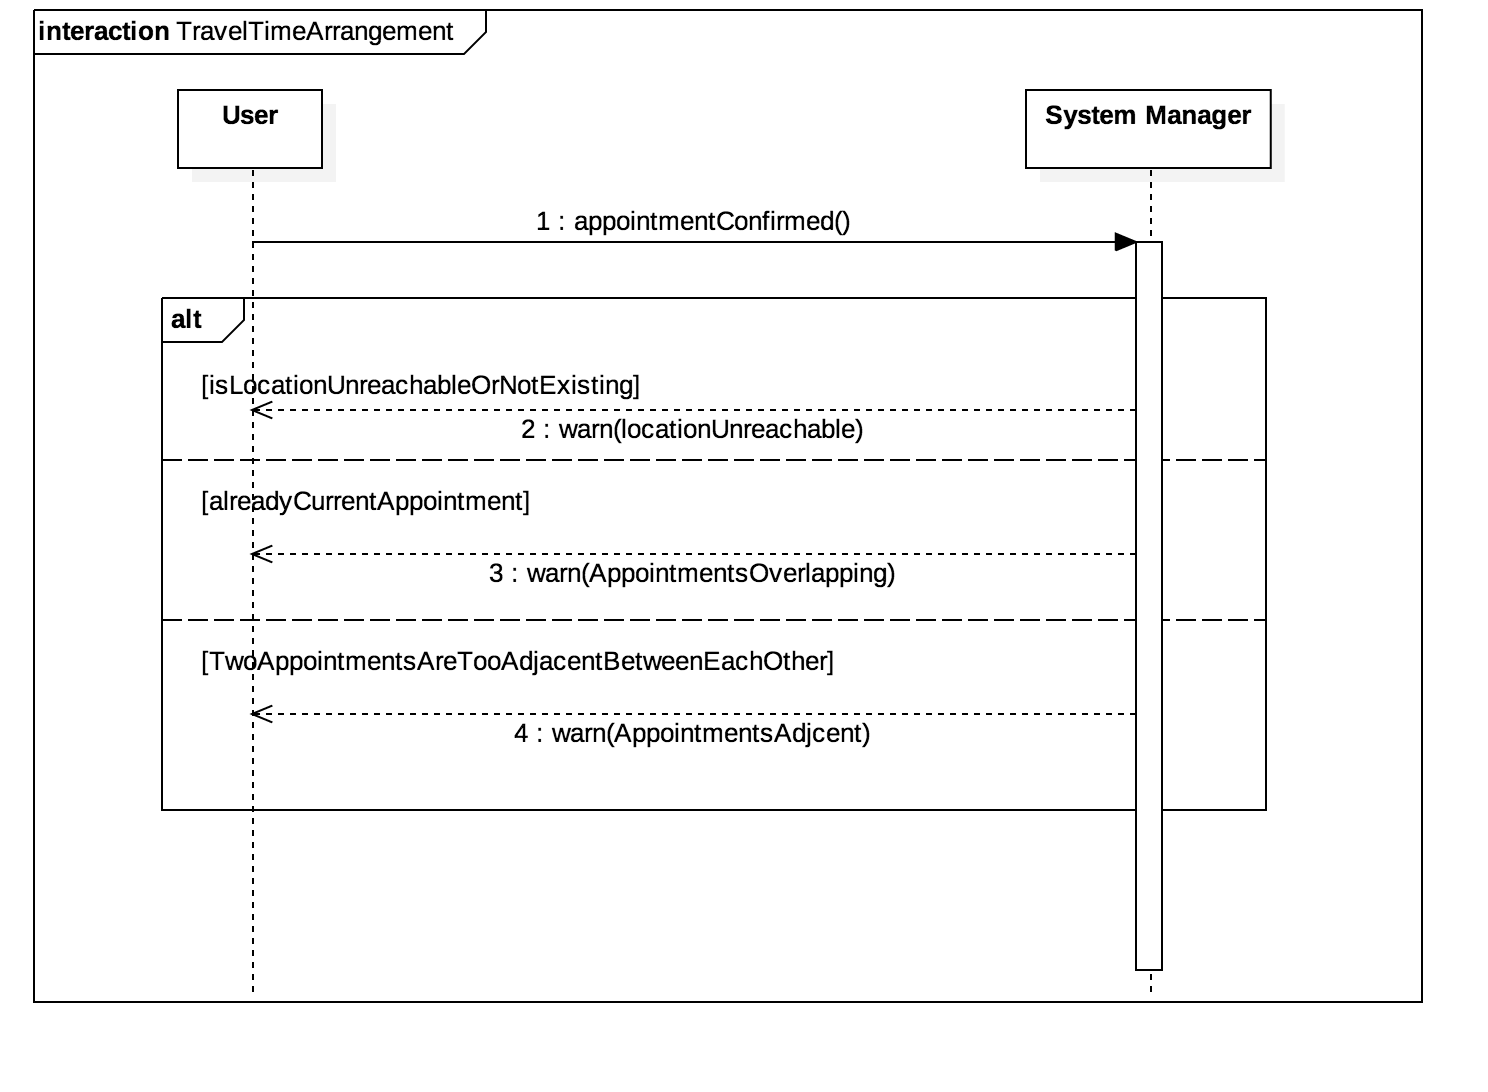
\includegraphics[width=6in]{./diagrams/TravelTimeArrangement.png}
	\caption{Sequence Diagram: Travel Time Arrangement.}
	\label{fig:TravelTime}
\end{figure}

\subsubsection{Statechart}
The statechart of the action undertaken by the system is illustrated in Figure \ref{fig:StateChecks}.
\begin{figure}
	\centering
	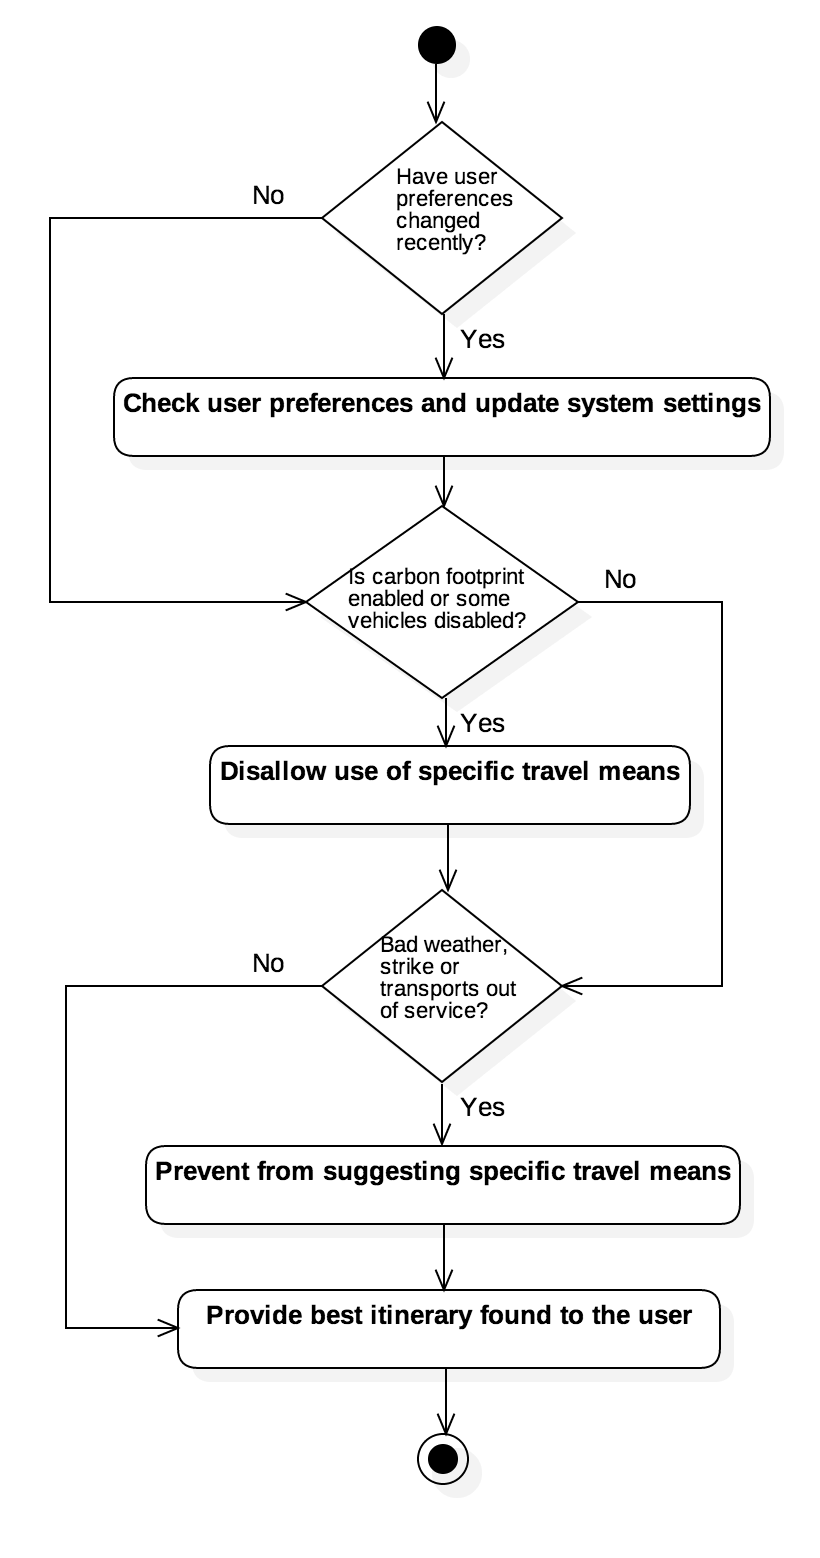
\includegraphics[width=5in]{./diagrams/StatechartChecks.png}
	\caption{Statechart: Travel Time Arrangement.}
	\label{fig:StateChecks}
\end{figure}

\subsubsection{Associated functional requirements}
\begin{enumerate}
\item The system will ask the user the first time to authorize the use geolocalization (estimation of the current position).
\item The system calculates the best itinerary only for events for the current day. Events for the following days, after being added to the calendar, are actually evaluated only when that specific day comes.
\item The system takes into account the current position as starting point by default.
\item The system allows the user to customize travel means to be taken according to his/her preferences.
\item The system computes the best route based on both user preferences and on factors which cannot be controlled by the user (belong to the external world).
\begin{itemize}
\item The system checks user preferences every time they have been changed.
\item The system disallows using car if the user is not 18-year-old yet.
\item The system will not provide a route with a specific transport, if the user has chosen not to use it.
\item The system will locate the nearest bike sharing system if the user is accustomed to riding a bike and favourable conditions occur.
\item The system will be likely to suggest walking instead of using motor vehicles if distance may take a little bit longer on foot but there's traffic jam.
\item The system will unlikely suggest walking if it is going to start raining.
\item The system will unlikely suggest car or taxis if the user has enabled carbon footprint optimization option.
\end{itemize}
\item The system will notify the user - when an event is approaching - that car can be taken if traffic is pretty much smooth, or underground train will be near there within few minutes, if the user is close to a station.
\item The system will reserve at least half an hour for lunchtime, or any other kind of breaks - if requested by the user.
\end{enumerate}

\subsubsection{Mockup}
The mockup of the itinerary resolved with navigation with car is shown in Figure \ref{fig:MockupMapCar}, whereas the itinerary with navigation with public transports is shown in Figure \ref{fig:MockupMapPt}. The mockup of settings preferences is shown in Figure \ref{fig:MockupSettings}. Finally, the mockup of notifications provided by the application is shown in Figure \ref{fig:MockupNotifications}.
\begin{figure}
	\centering
	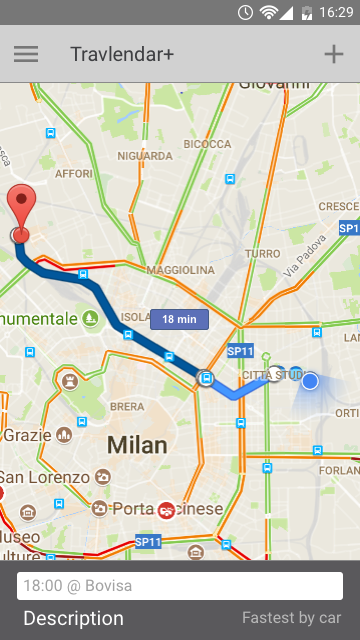
\includegraphics[width=4.5in]{./images/map_car.png}
	\caption{Navigation with car mockup.}
	\label{fig:MockupMapCar}
\end{figure}

\begin{figure}
	\centering
	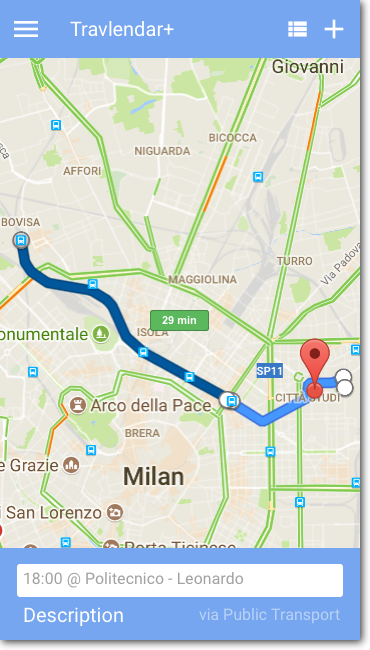
\includegraphics[width=4.5in]{./images/map_pt.png}
	\caption{Navigation with public transports mockup.}
	\label{fig:MockupMapPt}
\end{figure}

\begin{figure}
	\centering
	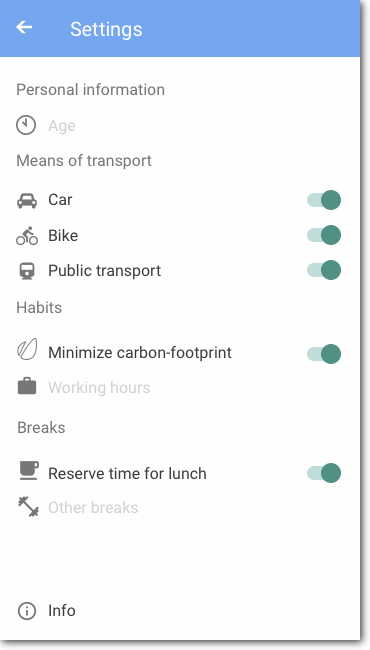
\includegraphics[width=4.5in]{./images/settings.png}
	\caption{User preferences settings mockup.}
	\label{fig:MockupSettings}
\end{figure}

\begin{figure}
	\centering
	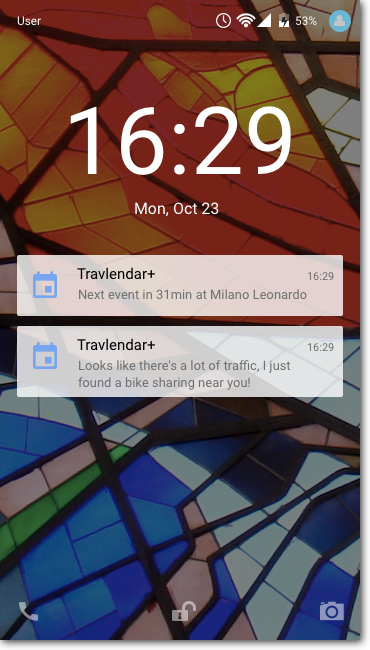
\includegraphics[width=4.5in]{./images/lockscreen.png}
	\caption{Application notification mockup.}
	\label{fig:MockupNotifications}
\end{figure}
\vspace*{26\baselineskip}